\section*{Problema 17.39, S}


Un avión supersónico que viaja a Mach $3$ a una altura de $20000m$ está directamente arriba de una persona en el tiempo $t = 0$, como se muestra en la figura. $a)$ ¿En qué tiempo la persona encontrará la onda de choque? $b)$ ¿Dónde estará el avión cuando finalmente se escuche el "estallido"? Tome la rapidez del sonido como $335m/s$.

\begin{figure}[H]
	\centering
	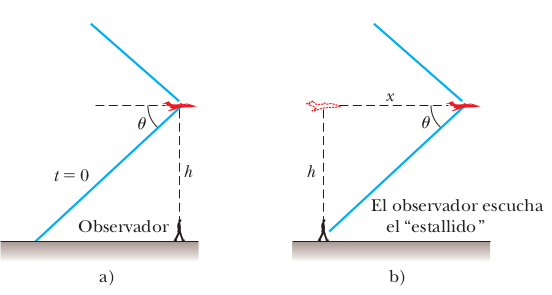
\includegraphics[scale=0.5]{./img/choqueonda.png}
	\label{choqueonda}
\end{figure}





%%%%